\documentclass[a4paper, 11pt]{report}
\author{Valentin Clement}
\title{CLAW FORTRAN Compiler - Developer's Guide}

\usepackage[utf8]{inputenc}
\usepackage{verbatim}
\usepackage{moreverb}
\usepackage[english]{babel}
\usepackage[T1]{fontenc}
\usepackage{lmodern}
\usepackage{graphicx}
\usepackage{fancyhdr}
\usepackage{listings}
\usepackage{lastpage}
\usepackage[top=2cm, bottom=1cm, left=2cm, right=2cm]{geometry}
\usepackage{color}
\usepackage[table]{xcolor}
\usepackage{graphicx}
\usepackage{lipsum}
\usepackage{pgfplots}
\usepackage{CJKutf8}
\usepackage{glossaries}
\usepackage{xspace}


\setcounter{secnumdepth}{3}

\def\fortran{FORTRAN\xspace}
\def\clawfcomp{CLAW FORTRAN Compiler\xspace}
\def\omni{OMNI Compiler\xspace}
\def\xcodeml{XcodeML/F\xspace}
\def\ffront{\lstinline!F_Front!\xspace}
\def\fback{\lstinline!F_Back!\xspace}
\def\fpp{\lstinline!FPP!\xspace}
\def\clawfc{\lstinline!clawfc!\xspace}
\def\cx2x{\lstinline!CX2X!\xspace}

\makeglossaries

\newacronym{ast}{AST}{Abstract Syntax Tree}
\newacronym{ir}{IR}{Intermediate Representation}


%font change
\renewcommand{\familydefault}{\sfdefault}

\newcommand{\HRule}{\rule{\linewidth}{0.5mm}}
\newcommand{\nl}{\\[0.1cm]}
\newcommand{\s}{\vspace{0.3cm}}
%\newcommand{\emptypage}{\newpage \thispagestyle{empty} \mbox{}\newpage}
\newcommand{\emptypage}{}
\newcommand{\smore}{\vspace{0.6cm}}

\usepackage{caption}
\DeclareCaptionFont{white}{\color{white}}
\DeclareCaptionFormat{listing}{\colorbox{gray}{\parbox{\textwidth}{#1#2#3}}}
\captionsetup[lstlisting]{format=listing,labelfont=white,textfont=white}

\definecolor{darkgreen}{rgb}{0,0.4,0}
\definecolor{mauve}{rgb}{0.58,0,0.82}
\definecolor{Gray}{rgb}{0,0,0}
\definecolor{LightGray}{gray}{0.9}


\lstset{
    basicstyle=\footnotesize\ttfamily,
    keywordstyle=\color{orange}, %keywordstyle=\color{MidnightBlue}\bfseries,
    identifierstyle=\color{black},
    commentstyle=\color{darkgreen},
    stringstyle=\color{red},
    numbers=left,
    numberstyle=\color{Gray}\tiny,
    frame=bt, %frame=single,
    rulecolor=\color{Gray},
    numbersep=7pt,
    extendedchars=true,
    captionpos=b,
    breaklines=true,
    showspaces=false,
    showtabs=false,
    tabsize=2,
    xleftmargin=20pt,
    framexleftmargin=20pt,
    framexrightmargin=0pt,
    framextopmargin=0pt,
    framexbottommargin=0pt,
    showstringspaces=false,
    aboveskip=20pt,
    belowskip=20pt
}

\lstset{
	emph={parclass, sync, async, broadcast, scatter, gather, reduce, seq, conc, mutex},
	emphstyle={\color{orange}\bfseries}
}

\addto\captionsenglish{%
  \renewcommand{\listfigurename}{List of figures}%
	\renewcommand\refname{}
}

%Header and footer
\pagestyle{fancy}
\fancyhead{}
\fancyfoot{}

%Header definition
\renewcommand{\headrulewidth}{0.5pt}
\lhead{CLAW FORTRAN Compiler}
\rhead{Developer's Guide}

%Footer definition
\renewcommand{\footrulewidth}{0.5pt}
\lfoot{Version 0.1}
\rfoot{Page \thepage ~on \pageref{LastPage}}

\definecolor{grey}{rgb}{0.9,0.9,0.9} 
% Color of the box surrounding the title - these values can be changed to give 
% the box a different color	

%remove indent for paragraph
\parindent0ex

\begin{document}

\thispagestyle{empty} % Remove page numbering on this page

%------------------------------------------------------------------------------
%	TITLE SECTION
%------------------------------------------------------------------------------
\colorbox{grey}{
	\parbox[t]{1.0\linewidth}{
		\centering \fontsize{35pt}{80pt}\selectfont 
		% The first argument for fontsize is the font size of the text and the 
		% second is the line spacing - you may need to play with these for your 
		% particular title
		
		\vspace*{2cm} 
		% Space between the start of the title and the top of the grey box
		
		\hfill \textbf{CLAW FORTRAN Compiler} \\
		\hfill Developer's Guide\par
		
		\vspace*{2cm} 
		% Space between the end of the title and the bottom of the grey box
	}
}

\vfill

\begin{center}

\includegraphics[width=4cm]{resources/c2sm_logo.pdf} \\
\end{center}

\vfill % Space between the title box and author information

\begin{center}
Version 0.1, Last updated \today \\
Author: Valentin Clement
\end{center}
\HRule

\clearpage % Whitespace to the end of the page



\newgeometry{top=3cm,bottom=3cm,right=2cm,left=2cm}

%\emptypage
%\pagebreak
%\label{chapter:ack}
%\begin{center}
%\textsc{\LARGE Acknowledgment}
%\end{center}
%\input{acknowledgment}

%\emptypage
%\pagebreak
%\label{chapter:abstract}
%\begin{center}
%\textsc{\LARGE Abstract}
%\end{center}


\emptypage
\pagebreak
\tableofcontents

\chapter*{Introduction}
This document describes the internal and external components of the \clawfcomp.
It gives an in-depth overview of the architecture of the compiler as well as 
the implementation of new transformations. 

\section*{Conventions used in this document}

Keywords and punctuation that are part of the actual specification will appear 
in typewriter font: \\

\lstinline|!$claw|\\

Italic font is used where a keyword or other name must be used: \\

\lstinline|!$claw| \textit{directive-name}\\

Optional syntax is enclosed in square brackets; an option that may be repeated
more than once is followed by ellipses:\\

\lstinline|!$claw| \textit{directive-name} [\textit{clause} [[,] \textit{clause}]. . . ]


\chapter{Architecture}
\section{OMNI Compiler}
The \clawfcomp is based on the \omni\cite{omni:website}. The \omni Project 
provides a set of programs to build source-to-source translator for C/C++ 
and FORTRAN. It is jointly developed by the Programming Environment Research 
Team of the RIKEN AICS and the HPCS Lab. of the University of Tsukuba both 
located in Japan. In the case of the \clawfcomp, we are using only the FORTRAN 
capabilities of the \omni. The FORTRAN front-end and back-end are still 
actively developed as of today and contribution can be made on their master 
repository\cite{omni:github}. 

\subsection{The FORTRAN front-end}
The FORTRAN front-end is the program that parses FORTRAN source code and that 
generates the \gls{ir}. Its grammar is written in \lstinline|yacc| and the 
processing and \gls{ir} generation is written in \lstinline|C|. This program 
can be called individually as shown in listing \ref{lst:ffront}.

\begin{lstlisting}[label=lst:ffront, language=Bash, caption=Call F\_Front]
F_Front -M my_module_dir -o my_program.xml my_program.f90
\end{lstlisting}

As the \omni acts as a compiler, it also has a notion of module. When a FORTRAN
module is parsed with the front-end, a \lstinline|.xmod| file is generated. 
This file contains all the signatures included in the module. This file is then 
needed to parse other FORTRAN code depending on the module.

\begin{lstlisting}[label=lst:m1, language=Fortran, caption=module\_m1.f90]
MODULE m1
  USE m2
END MODULE m1
\end{lstlisting}

\begin{lstlisting}[label=lst:m2, language=Fortran, caption=module\_m2.f90]
MODULE m2
  USE m3
END MODULE m2
\end{lstlisting}

\begin{lstlisting}[label=lst:m3, language=Fortran, caption=module\_m3.f90]
MODULE m3
END MODULE m3
\end{lstlisting}

If we take the simple example shown in listings \ref{lst:m1}, \ref{lst:m2} and 
\ref{lst:m3}, where we have a module 1 depending on module 2 and module 2 
depending on module 3. These source files should be processed by the front-end
as shown in listing \ref{lst:ffrontdep}.

\begin{lstlisting}[label=lst:ffrontdep, language=Bash, caption=Parse module with dependencies]
F_Front -o module_m3.xml module_m3.f90      # produces m3.xmod
F_Front -M . -o module_m2.xml module_m2.f90 # uses m3.xmod and produces m2.xmod
F_Front -M . -o module_m1.xml module_m1.f90 # uses m2.xmod and produces m1.xmod
\end{lstlisting}


\subsection{\xcodeml}
\xcodeml\cite{omni:xcodemlf95,omni:xcodemlf2008} is the \gls{ir} used by the 
translator in the CLAW FORTRAN Compiler. This \gls{ir} is based on the XML
format and is described in a specification document. It allows to have an
high-level representation of FORTRAN 2008 programs.

Listing \ref{fortran1} is a simple FORTRAN program. Its \xcodeml \gls{ir} is 
shown in listing \ref{xcodeml1}. A typical \xcodeml translation unit is
composed of the followings sections: 
\begin{itemize}
\item Type table with all the type definitions used in the translation unit
(Listing \ref{xcodeml1} line 6-24).
\item Global symbols table listing all the symbols at global scope (Listing
\ref{xcodeml1} line 25-29).
\item Global declarations section listing the actual function and/or module
declarations (Listing \ref{xcodeml1} line 30-82).
\end{itemize}

\lstinputlisting
  [
    label=fortran1, 
    caption=Basic FORTRAN program, 
    language=Fortran
  ]{code/basic_fortran.f90}

\lstinputlisting
  [
    label=xcodeml1, 
    caption=\xcodeml IR, 
    language=xml
  ]{code/basic_fortran.xml}

\subsection{The FORTRAN back-end}
The FORTRAN back-end is the program that decompiles \gls{ir} back to FORTRAN 
code. It is a simple Java program that implements a visitor patterns across 
the \gls{ast}. It can be called as a standalone program or directly within the
translator as it is done in the \clawfcomp.

\section{\clawfcomp}

The \clawfc is the program handed to the end-user. It performs all the needed 
step to have a source-to-source translation of a FORTRAN program. As shown in 
Figure \ref{fig:clawfc_main_workflow}, it is composed by various programs 
under-the-hood. The complete workflow is devided as follows: 

\begin{enumerate}
\item \textbf{FPP}: The FORTRAN source code is preprocessed by a standard 
FORTRAN preprocessor. Typically the one provided by the default compiler. 
The \lstinline|FC| environment variable is used by the CMake build system to 
determine it.
\item \textbf{F\_Front}: The preprocessed FORTRAN source code is then parsed 
by the OMNI Compiler FORTRAN Front-end to produce the input \xcodeml \gls{ir}.
\item \textbf{CX2X}: The input \xcodeml \gls{ir} is manipulated according to 
the rules of the CLAW directive language. It produces the output \xcodeml 
\gls{ir}.
\item \textbf{F\_Back}: The output \xcodeml \gls{ir} is analyzed to produce 
the transformed FORTRAN code. 
\end{enumerate}

\ffront{}, \fback{} are part of the \omni{}, \fpp{} is provided by the 
installed FORTRAN compiler. The \xcodeml to \xcodeml translator \cx2x{} is 
actively developed as part of the CLAW project.  

\begin{figure}[!ht]
  \centering
  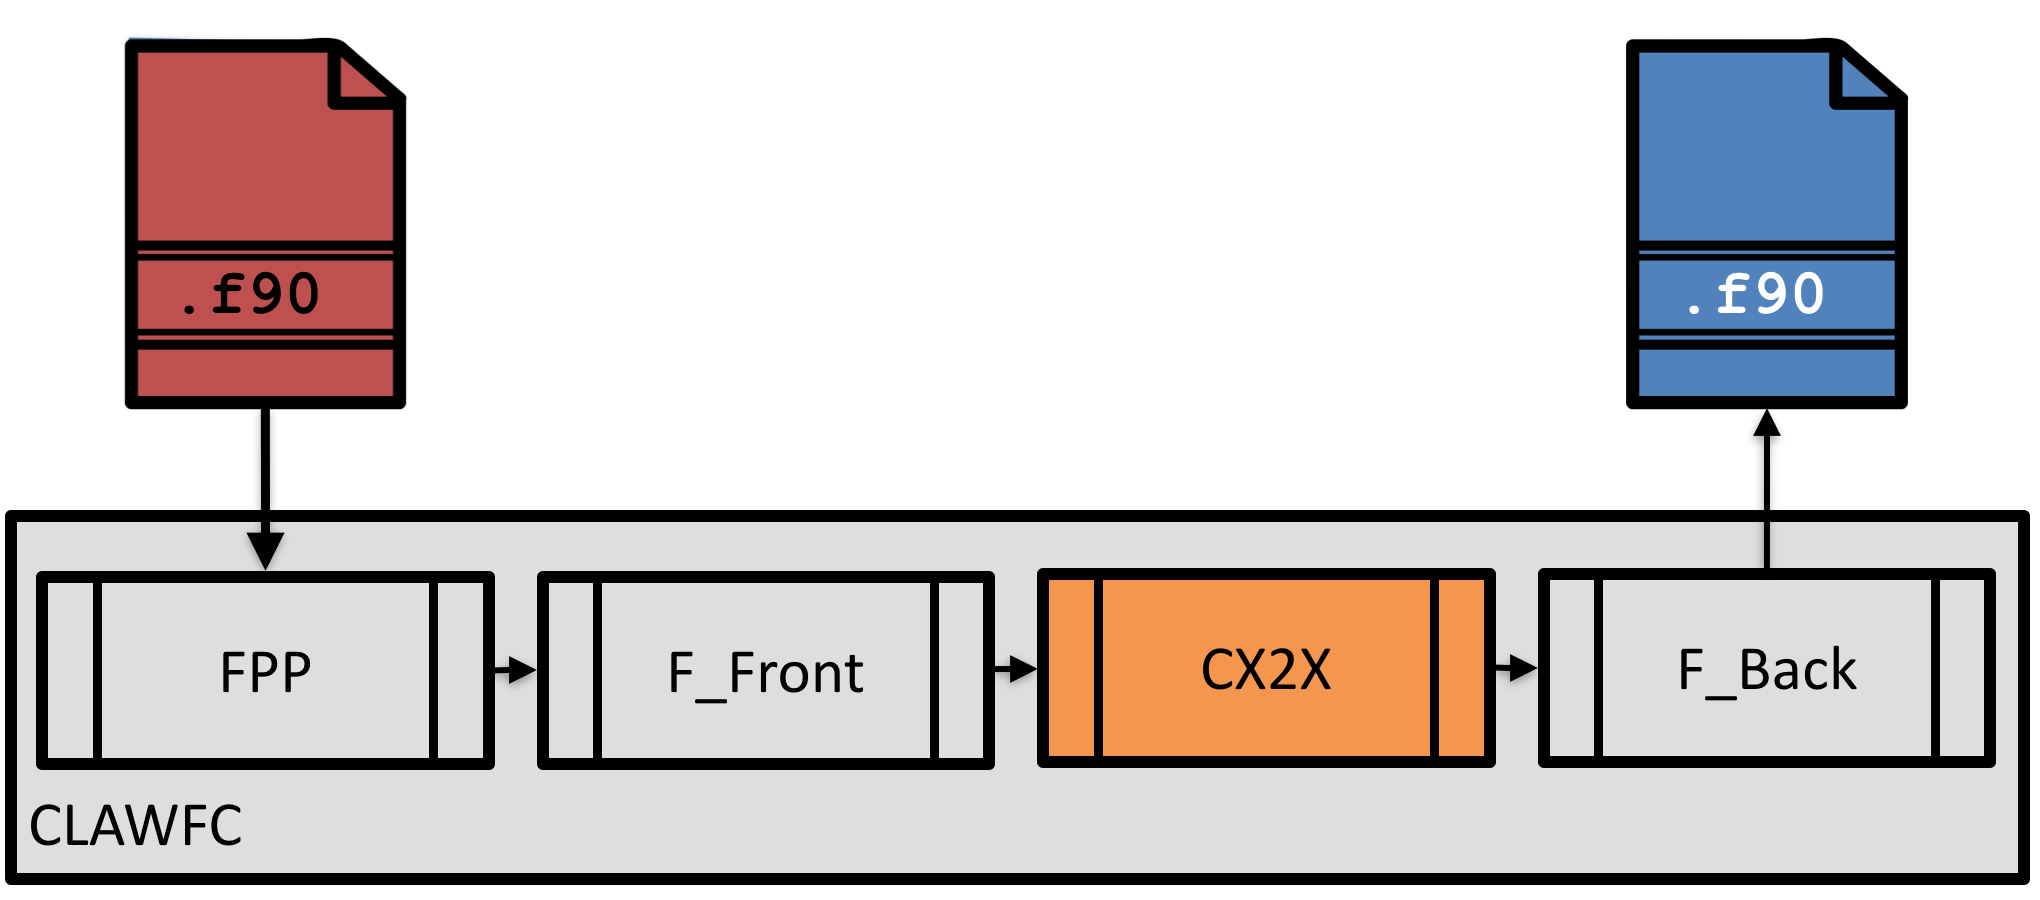
\includegraphics[
    width=0.8\textwidth
  ]{resources/clawfc_global_workflow.png} \\
  \caption{CLAW FORTRAN Compiler main workflow.}
  \label{fig:clawfc_main_workflow}
\end{figure}

\section{CLAW \xcodeml to \xcodeml translator}
The \xcodeml to \xcodeml translator is the intelligence of the \clawfcomp. It 
understands the CLAW directive language and apply the corresponding 
transformation to the \xcodeml \gls{ast}.

\begin{figure}[!ht]
  \centering
  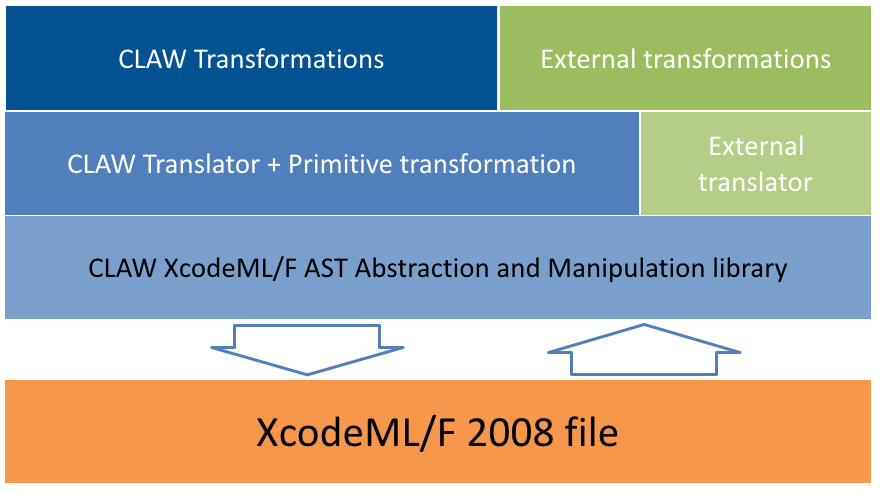
\includegraphics[width=0.8\textwidth]{resources/cx2x_stack.png} \\
  \caption{CLAW \xcodeml to \xcodeml library stack.}
  \label{fig:cx2x_stack}
\end{figure}

Figure \ref{fig:cx2x_stack} shows the stack of libraries used in the the CLAW 
\xcodeml to \xcodeml translator. The two first layers from the bottom are 
explained in more details in chapter \ref{chapter:astmanip}. The three last 
layers are explained in chapter \ref{chapter:transformation}.


\chapter{CLAW directive language}
%TODO add ref for the document
The CLAW directive language is specified in the "CLAW directive language 
specification". To validate and understand this language, a parser is needed 
in the heart of the \clawfcomp.

\section{CLAW directive language parser}
%TODO add ref to ANTLR
The CLAW directive language parser is based on the ANTLR project
\cite{Parr:2013:DAR:2501720}. ANTLR is a parser generator. From a grammar file,
ANTLR generates a parser that is then used in the CLAW \xcodeml to \xcodeml 
translator to interpret the directives. 

\lstinputlisting
  [
    label=lst:antlr, 
    language=Java, 
    caption=ANTLR Grammar Example
  ]{code/clawp.g4}

Listing \ref{lst:antlr} is a minimalist ANTLR example that support only two 
directives \lstinline|!$claw acc| or \lstinline|!$claw omp|.

In this grammar, there are two important sections, the parser and the lexer 
sections. The lexer section defined what will be recognized as a token. Here 
we defined the directives, the clauses but also more complex construct such as 
the \lstinline|IDENTIFIER| on line 28. It described the possible element to 
compose an identifier. This \lstinline|IDENTIFIER| can then be used later in 
the parser rules. 
The parser rules are defining the actual grammar of the language. In the case 
of this small example, the grammar says that the directive string must begins 
with \lstinline|claw| and then be followed by \lstinline|acc| or 
\lstinline|omp|. The code in \lstinline|{}| is java code that is triggered 
when the grammar rule is activated. In the example, it sets a value of the 
object returned after the analysis.
The \lstinline|@init{}| section allows to execute some Java code before 
triggering the actual parse. The \lstinline|@header{}| allows to insert Java 
code before the parser class.

\begin{lstlisting}[label=lst:antlr_cmd, caption=ANTLR parser generation command, language=bash]
javac -classpath <antlr_jar> org.antlr.v4.Tool -o . -package cx2x.translator.language.parser Claw.g4
\end{lstlisting}

The full CLAW ANTLR grammar is defined in the following file: 
\lstinline|omni-cx2x/src/cx2x/translator/language/parser/Claw.g4|

\chapter{Transformation}
\label{chapter:transformation}
A transformation class is the the basic representation of a manipulation of the
\gls{ast} triggered by a directive. Each directive is implemented in its own 
transformation class. If the directive can be used as a block directive (with a
\lstinline|!$end <directive>| directive), the class must inherits from the 
\lstinline!ClawBlockTransformation!. Otherwise, it can inherits from the basic 
\lstinline!ClawTransformation! class.

\section{Type of transformation}
Transformations are divided into two distinct groups. The independent and the 
dependent transformations. The first one, as its name implies, is performed 
independently of any other transformations. The dependent transformation, in the
other hand, is applied only when it can be combined with another dependent 
transformation of the same kind in its group. Most of the transformations are 
independent. The best example for the dependent transformation is the loop 
fusion transformation. As shown in Listing \ref{lst:trans_dep}, there are two 
CLAW directives (line 4 and 9). These directives will trigger two dependent loop
fusion transformations. Alone, those transformations have no effect
on the \gls{ast}. The transformation engine will analyze if the 
first one can be transformed with the second one. If so, the transformations will
be grouped together and the fusion will happen. Otherwise, the transformations 
are just ignored as they have to depend on at least one other transformation.

\lstinputlisting
  [
    label=lst:trans_dep, 
    caption=Loop fusion example, 
    language=Fortran
  ]{code/trans_dependent.f90}

\section{Transformation application order}
The first step of the transformation of a translation unit (an XcodeML/F file), 
is the detection of all the CLAW directives. Each directive will trigger the 
creation of an instance of the transformation class it belongs to. For example,
a loop-fusion directive will trigger the creation of a \lstinline|LoopFusion| 
instance. On this instance, the \lstinline|analyze| method is called in order 
to determined if the transformation can take place. If the analysis step is 
successful, the transformation is added to its transformation group. 
Once all the transformation instances have been analyzed and categorized by 
groups, the actual code transformation can take place on the AST. All 
transformations in a group are applied one after another in a FIFO order. 
The order in which groups are processed is determined by the CLAW configuration
file.

\lstinputlisting
  [
    label=lst:config, 
    caption=CLAW default configuration, 
    language=xml
  ]{code/claw-default.xml}

As shown in Figure \ref{lst:config}, the transformation order is specified the
configuration file under the XML format.
Each transformation group is defined with its type (dependent or 
independent), its user-friendly name and its implementation class (class 
inheriting from \lstinline|ClawTransformation| or 
\lstinline|ClawBlockTransformation| and implementing the actual transformation
on the AST). The order of application is from top to down.


\section{Add a new transformation}
A transformation in the \clawfc is represented as a class that inherits from 
the \lstinline|ClawTranformation| or \lstinline|ClawBlockTransformation| 
base class. In order to add a new transformation into the the CLAW Compiler, 
the following steps must be done.

\begin{enumerate}
\item Create a new class that inherits from one of the base transformation 
      class.
\item Define the directive that will trigger the transformation and add it 
      to the CLAW language parser.
\item Detect and categorize the new transformation.      
\item Add the transformation to the configuration file.
\end{enumerate}

As an example, the next 4 subsection describe those steps with more details. 

\subsection{New transformation class}
The transformation created at this step will be a simple independent 
transformation. It will then inherits for \lstinline|ClawTransformation| class.

\lstinputlisting
  [
    label=lst:myfirsttransformation.java, 
    caption=MyFirstTransformation.java, 
    language=java
  ]{code/MyFirstTransformation.java}

The transformation class shown in Listing \ref{lst:myfirsttransformation.java}
is really simple. It just inherits from \lstinline|ClawTransformation| on line
16. Therefore, it has to implements the \lstinline|analyze|, 
\lstinline|transform| and \lstinline|canBeTransformedWith| methods as they are 
abstract in the base class. 

The \lstinline|analyze| method does not perform any check and just return 
\lstinline|true| to tell the transformation engine that the actual 
transformation can occur. 

The \lstinline|transform| method is pretty simple. It delete the pragma that 
triggered the transformation from the \gls{ast}. It will then not be in the 
resulting transformed code.

\subsection{Directive and CLAW language parser}

\subsection{Detection and categorization}

\subsection{Enable the new transformation}



\chapter{\xcodeml and AST manipulation library}
\label{chapter:astmanip}
As the \xcodeml \gls{ir} is based on the XML format, it can be manipulated with
any language that can read and write XML files. It can even be manipulated by 
hand depending on the user's knowledge of the \xcodeml \gls{ir} specification. 
To ease this task, a small manipulation library is included in the \cx2x 
program. This library helps to traverse the \gls{ast}, add, modify or delete 
node.

\section{Traverse the \gls{ast}}

\section{Add nodes}

\begin{lstlisting}[label=lst:add_node, language=Java, caption=XcodeML/F add node example]
public void transform(XcodeProgram xcodeml, Transformer transformer,
                      Transformation other)
{                      
    Xnode myNewNode = new Xnode(xcodeml, Xcode.FPRAGMASTATEMENT);
    myNewNode.setValue("omp parallel");
    XnodeUtil.insertAfter(_claw.getPragma(), myNewNode);
}
\end{lstlisting}

\section{Modify nodes}

\begin{lstlisting}[label=lst:update_node, language=Java, caption=XcodeML/F update node example]
public void transform(XcodeProgram xcodeml, Transformer transformer,
                      Transformation other)
{                      
    Xnode pragma = _claw.getPragma();
    // Get current values from the node
    String oldValue = pragma.value();
    int line = pragma.lineNo();
    // Update the value directly in the AST
    pragma.setValue("acc routine seq");
    pragma.setLineNo(line + 1);
}
\end{lstlisting}

\section{Delete nodes}
\begin{lstlisting}[label=lst:delete_node, language=Java, caption=XcodeML/F delete node example]
public void transform(XcodeProgram xcodeml, Transformer transformer,
                      Transformation other)
{                      
    Xnode pragma = _claw.getPragma();
    pragma.delete(); // Delete the node in the AST
}
\end{lstlisting}


% GLOSSARY
\pagebreak
\glsaddall
\printglossaries

\emptypage
% FIGURES
\pagebreak
\listoffigures

%TABLES
\pagebreak
\listoftables

\emptypage
% LISTINGS
\pagebreak
\lstlistoflistings

% REFERENCES
\bibliography{developers_guide} 
\bibliographystyle{ieeetr}


%\emptypage
%\input{appendix}

\end{document}
